\section{RAMNet}
\textit{Recurrent Attention Models} iteratively attends to different parts of the input sequence over multiple time steps, adjusting its focus based on the task at hand.

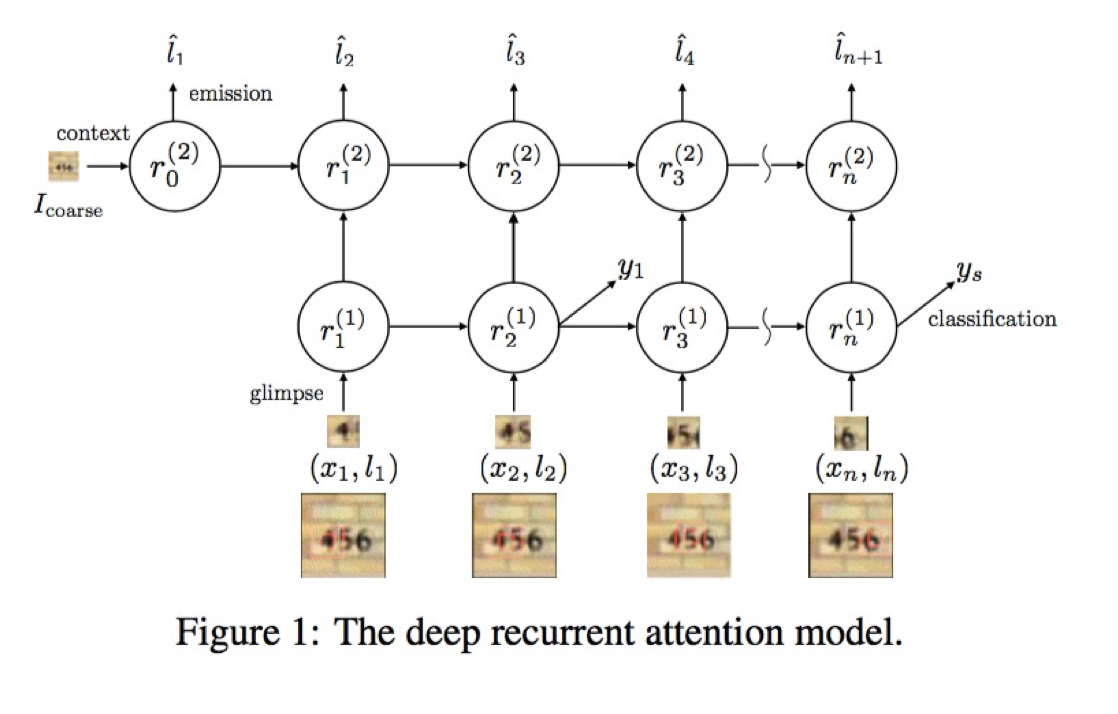
\includegraphics[width=0.9\columnwidth]{images/RAM.png}

We compare $y$ to target and backprop. Stop the gradient after the first mislabeled target. Choose random locations at first, and reward it for picking locations that work well. 

\section{Transformers}
Attention based methods (transformers) compute an attention vector dynamically, which is then used to gate the previous hidden states. Then during decoding, the decoder can choose to pay attention to any of the states of the encoder. Feed-forward. Replicate the network for every input. Fast to train. Can be used for images (encoder only). Takes in patches of an image without convolutions.

Reccurence-based methods have to wait since hidden states depend on all previous hidden states (i.e. can't take advantage of parallelism).
